\subsection{Sensitivity Analysis}
\label{exp:sensi}


%\begin{figure}
%	
%	\centering
%	\subfigure[The impact of alpha value]{
%		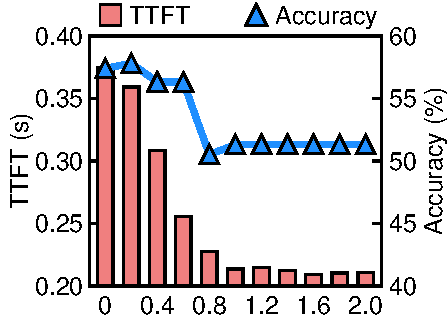
\includegraphics[width=1.5in, height=1.0in]{sensitivity.pdf}}
%	\hspace{0.06in}	
%	\subfigure[The impact of chunck size]{
%		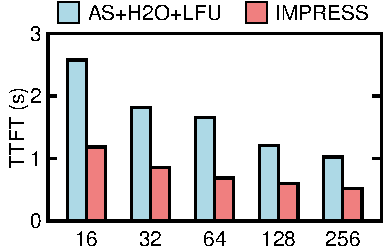
\includegraphics[width=1.5in, height=1in]{indiv_c_rte.pdf}
%	}
%	\vspace{-0.1in}
%	\caption{xxx}
%	\label{fig:sensitivity_alpha}
%\end{figure}

\noindent \textbf{Alpha value of similarity threshold.} 
% Figure~\ref{fig:sensitivity_alpha} shows the results for model inference accuracy and TTFT as the alpha value is adjusted from 0 to 2. 
% It shows that as the alpha value increases, TTFT decreases, but the model inference accuracy also drops. This is because a larger alpha value lowers the similarity threshold, making it easier for the similarity of the important token index sets in the probe heads to exceed the threshold, resulting in fewer KVs being loaded. (as discussed in \cref{sec:techa}). 
% Similar trends are observed across other datasets. 
% Therefore, we set alpha to 0.6 to achieve lower TTFT while maintaining high inference accuracy.
Figure~\ref{fig:sensitivity_alpha} depicts the impact of varying the alpha value on inference accuracy and TTFT, ranging from 0 to 2. The findings indicate that while an increased alpha reduces TTFT, it marginally affects inference accuracy due to a lowered similarity threshold, leading to less KV loading. This trend is consistent across datasets. Thus, we optimize alpha at 0.6 for a balance between low TTFT and high inference precision.

\noindent \textbf{Chunk size.} 
% Figure~\ref{fig:sens_ck} shows the TTFT results of the current state-of-the-art system and \pname{} as the chunk size is adjusted from 16 to 256. Since chunk size does not affect accuracy, we omit it from the figure. 
% We observe that across different chunk sizes, \pname{} consistently outperforms
% AS+H2O+LFU system by 2.2$\times$ to 2.4$\times$. This demonstrates the
% superiority of the \pname{} system under various chunk sizes.
Figure~\ref{fig:sens_ck} compares the TTFT of the leading system and \pname{} with chunk sizes ranging from 16 to 256. Notably, \pname{} achieves 2.2$\times$ to 2.4$\times$ improvement over the AS+H2O+LFU system across all sizes, underscoring \pname{}'s robustness regardless of chunk dimensions. Accuracy, being unaffected by chunk size, is not depicted.







\noindent 
\fv{
\textbf{Dataset size.}
%We varied the number of prefixes (i.e., few-shot examples) to create variants of the OpenBookQA with different dataset sizes from 65GB to 400GB. Figure~\ref{fig:sens_datasetsize} shows that \pname{} consistently outperforms the leading comparison systems with 
%the speedup of \pname{} varies from 1.2$\times$ to 2.0$\times$.
% increases from x$\times$ to y$\times$ as the 
% dataset grows from 65GB to 400GB compared to the leading baseline. This is because larger datasets exacerbate I/O bottlenecks, allowing \pname{} to achieve greater performance improvements.
We vary the number of prefixes (i.e., few-shot examples) to create different variants of OpenBookQA, with dataset sizes ranging from 65GB to 400GB. Figure~\ref{fig:sens_datasetsize} shows that \pname{} consistently outperforms the leading comparison system, AS+H2O+LFU, achieving speedups ranging from 1.2$\times$ to 2.0$\times$.
}

\noindent 
\fv{
\textbf{Model type.} 
Figure~\ref{fig:sens_modeltype} shows the average TTFT for Llama2-7B and Llama2-13B models on PIQA and COPA. It demonstrates that \pname{} achieves a 1.7$\times$-2.7$\times$ speedup on Llama models, attributed to similar reasons in~\cref{exp:overall}.
}

